\chapter{Results}
In this section we present and compare results of the four models aplied in STLF. The performance of the models are evaluated using MAPE, MAE, RMSE and R\^2. These metrics can give us a clear picture and comparisons framework for each of the model performance.  The goal is to represent the accuracy, robustness and suitability of the ML and AI models to solve STLF.

The metrics theory is explained in \ref{sec:eval_metrics} which shows the mathematics behind each of the metrics used in the research. The methodology shows the creation of the models and how these results were produced. 


\subsection{Dataset Results}
 The continuous\_dataset.csv contained well ordered data that was collected with minimum errors, empty data was filled using the forward and back-filling process.Figure \ref{fig:originaldataset}
 \begin{figure}[h]
 	\centering
 \begin{minipage}[b]{0.45\linewidth}
 	\centering
 	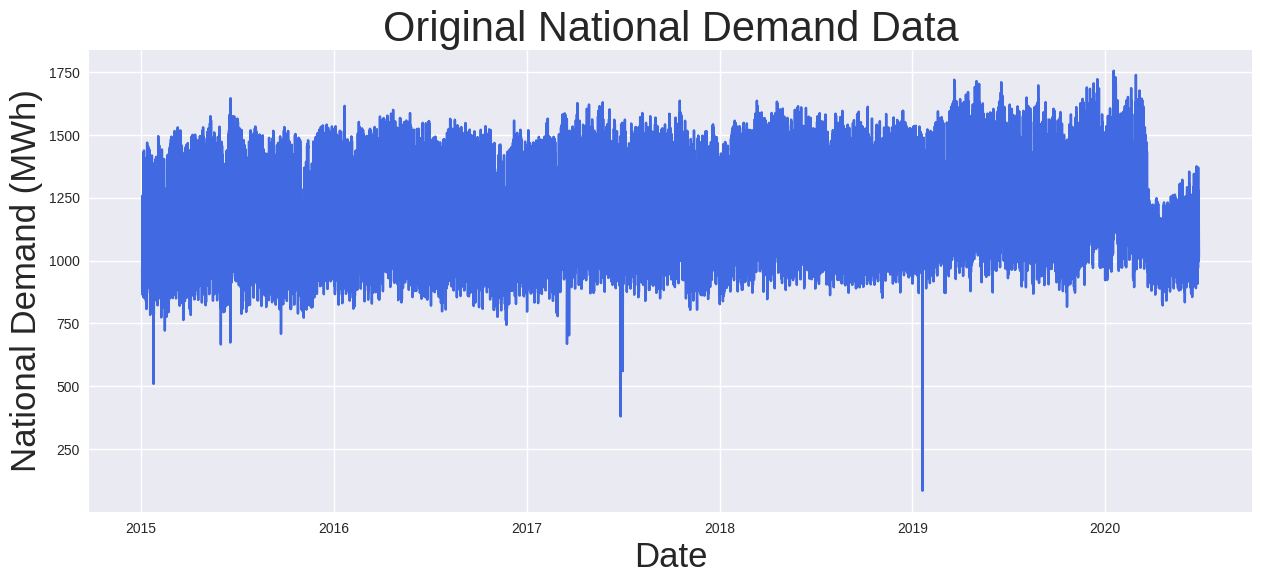
\includegraphics[width=\linewidth]{Chapters/images/results/original_dataset}
 	\caption{The original national demand .}
 	\label{fig:originaldataset}
 \end{minipage}
 \begin{minipage}[b]{0.45\linewidth}
 	\centering
 	\includegraphics[width=\linewidth]{"Chapters/images/results/train test split_after HI"}
 	\caption{HI processed dataset with traintest split.}
 	\label{fig:train-test-splitafter-hi}
 \end{minipage}
 \end{figure}
 
 The HI method explained in section \ref{sec:HI_method}, was used to handle outliers in the dataset, fixing all data-points that deviated from the normalcy presented in the dataset. After the implementation of the HI-method the train test split of 80/20 was implemented. Figure \ref{fig:train-test-splitafter-hi} shows the effectiveness of the HI method in removing noisy details in the dataset.

 \begin{figure}[h]
  	\centering
  	% First figure
  	\begin{minipage}[b]{0.45\linewidth}
  		\centering
  		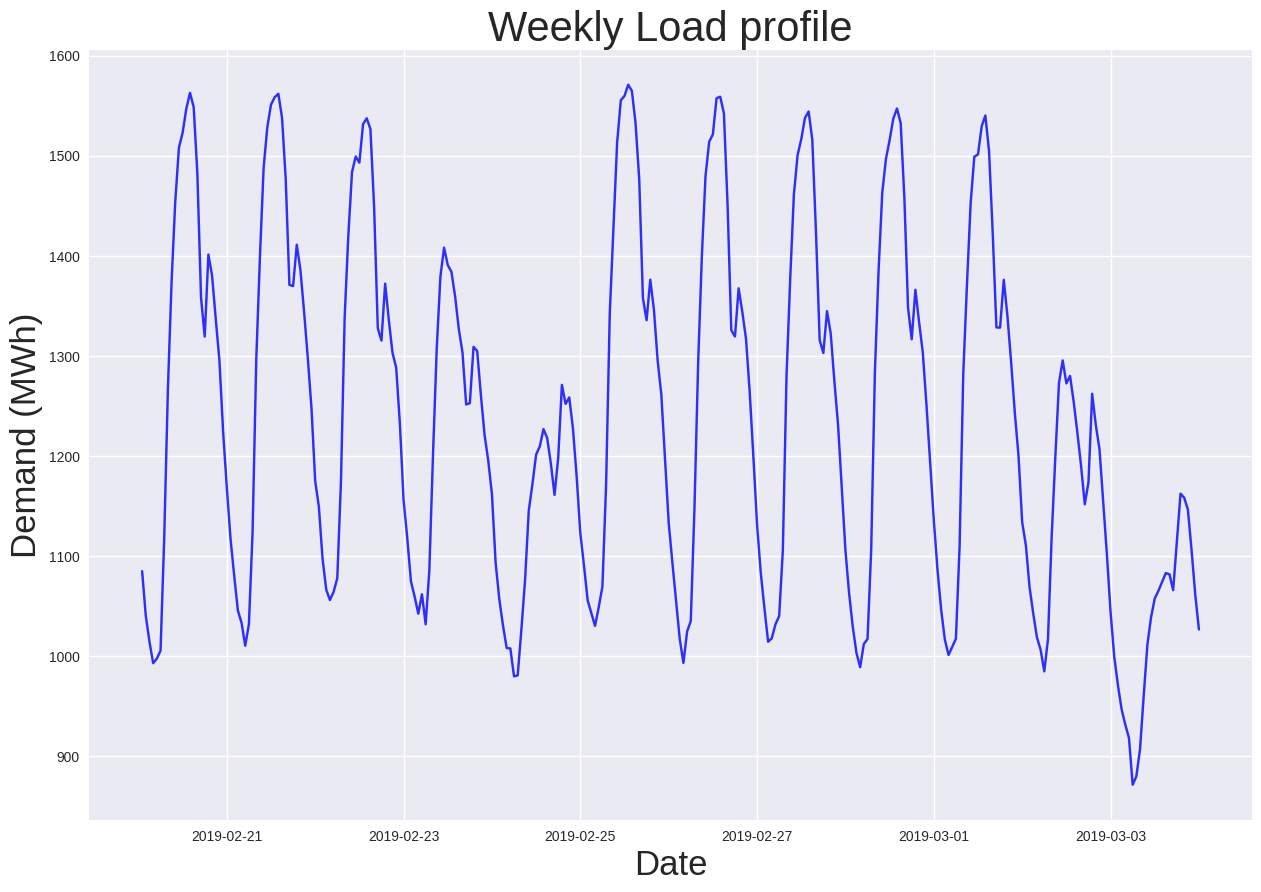
\includegraphics[width=\linewidth]{Chapters/images/results/weekly_load_profile.png}
  		\caption{The general weekly national load profile.}
  		\label{fig:weeklyloadprofile}
  	\end{minipage}
  	\hfill
  	% Second figure
  	\begin{minipage}[b]{0.45\linewidth}
  		\centering
  		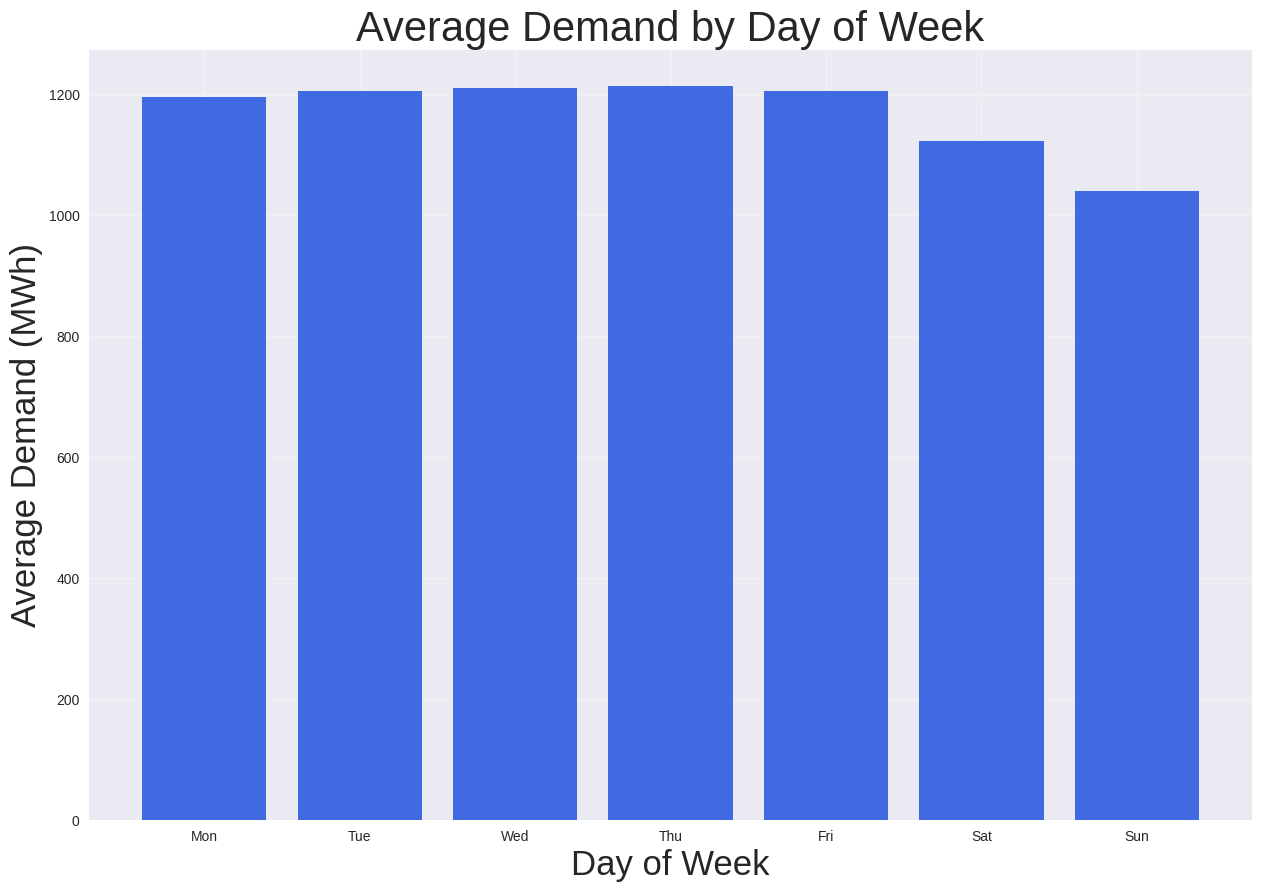
\includegraphics[width=\linewidth]{Chapters/images/results/average_daily_demand.png}
  		\caption{The weekly average daily demand }
  		\label{fig:averagedailydemand}
  	\end{minipage}
  \end{figure}
  
  
  To further understand the dataset, it was broken down to give the more insight on how the data and load behaves at different points. Firstly the weekly load profile in figure \ref{fig:weeklyloadprofile} shows a daily pattern that the load exhibits.The trend shows a higher usage during the week and lower usage in the weekend, with the lowest usage day being Sunday. 
  
  
  Figure \ref{fig:averagedailydemand} shows the average daily demand  of electricity. It also shows a higher usage during the week and lower consumption on the weekend, with Sunday being the lowest consumption day. 
  \begin{figure}[h]
  	\centering
  	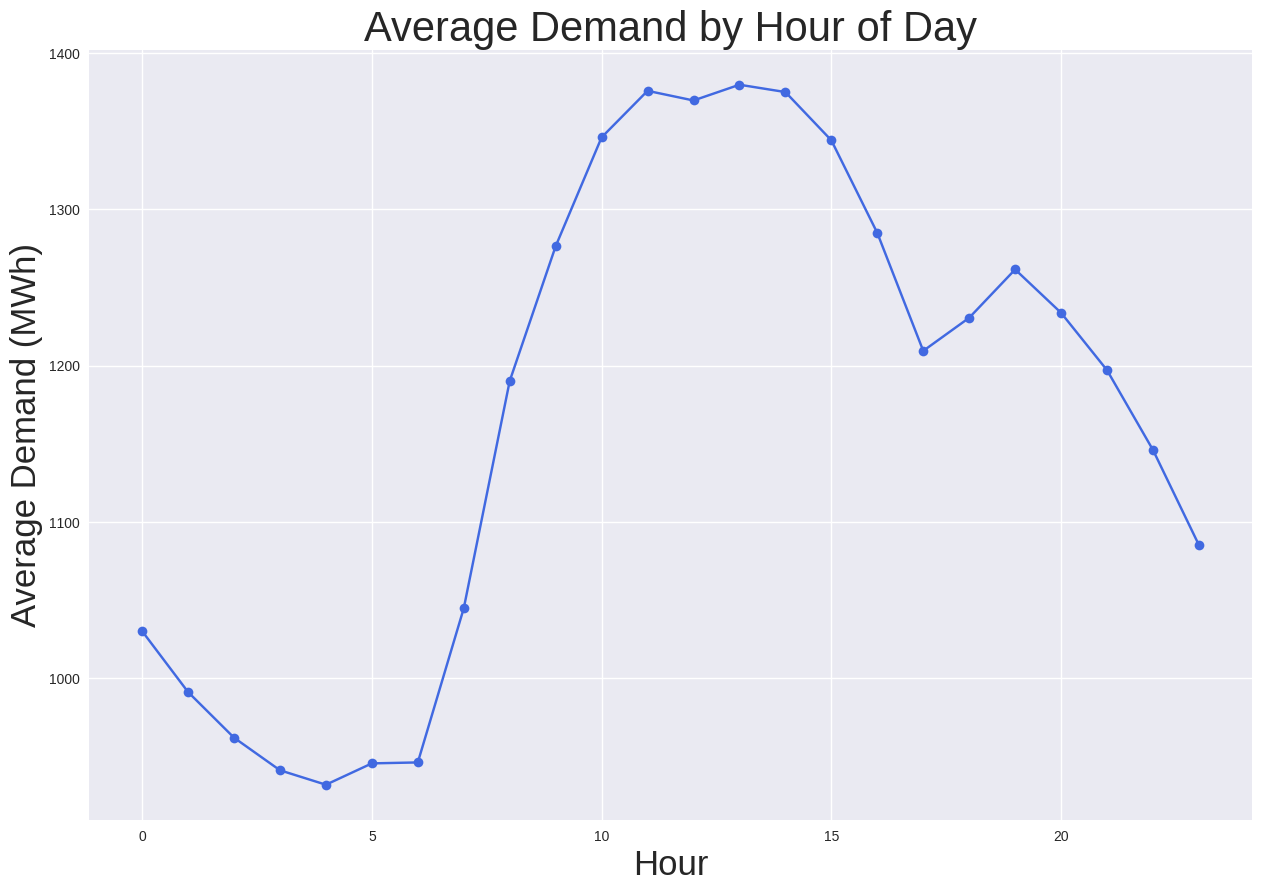
\includegraphics[width=0.45\linewidth]{Chapters/images/results/average_hourly_demand}
  	\caption{Average hourly demand of electricity between 2015 and 2020 in panama}
  	\label{fig:averagehourlydemand}
  \end{figure}
  
  Figure \ref{fig:averagehourlydemand} shows the average hourly usage of data. The averages show that the lowest consumption is in the early hours of the day, with a steady rise in the early morning leading to a peak at midday. After midday there is a steady decrease in demand with a slight increase between the 18th and 20th hour of the day, this is followed by a drop in usage leading to the early hours of the day.  


\subsection{Model Simulation Results}

\subsubsection{Exponential smoothing}
The models tested in the research were created using python and tensorflow, using google collab an cloud jupyter notebook environment for faster processing and version control through google drive. 

The ES model being the benchmark model achieved a MAPE of 9.57\% with a MAE of 118.18Mwh using the triple Multiplicative Damped model. Table \ref{tab:exp_smoothing_results} below contains the the results produced by the ES model and the parameters of the model. 
\begin{table}[h]
	\centering
	
	\begin{tabular}{ll}
		\hline
		\textbf{Metric / Parameter} & \textbf{Value} \\
		\hline
		\multicolumn{2}{l}{\textbf{Model Results}} \\
		AIC & 20118.40 \\
		MAPE &  9.57\% \\
		MAE & 118.14 \\
		RMSE & 141.84 \\
		Correlation & 0.7239\\
		\hline
		\multicolumn{2}{l}{\textbf{Model Parameters}} \\
		Smoothing Level ($\alpha$) & 1.0000 \\
		Smoothing Trend ($\beta$) & 0.0000 \\
		Smoothing Seasonal ($\gamma$) & 0.0000 \\
		Damping Trend ($\phi$) & 0.9744 \\
		Initial Level ($l_0$) & 1071.1459 \\
		Initial Trend ($b_0$) & 1.0236 \\
		Initial Seasons & [0.9093, 0.8828, 0.8638, 0.8555, 0.8682, ...] (shape = 24) \\
		Use Box-Cox & 0.0000 \\
		Lambda ($\lambda$) & None \\
		Remove Bias & 0.0000 \\
		\hline
	\end{tabular}
	\caption{Triple Multiplicative Damped Exponential Smoothing Model Parameters and Results}
	\label{tab:exp_smoothing_results}
\end{table}
These parameters produced the best results in comparison to other ES models and this was evaluated through the algorithm shown in  \ref{fig:exponential-smoothing-model-choice}. 
\begin{figure}[h]
	\begin{minipage}[b]{0.45\linewidth}
	\centering
	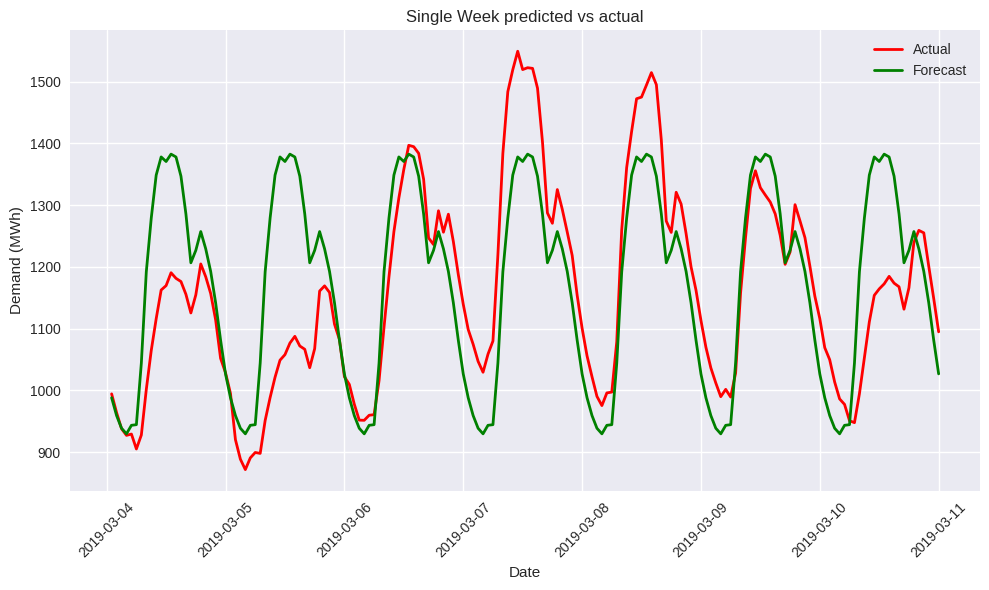
\includegraphics[width=\linewidth]{Chapters/images/results/ES_predicted_vs_actual}
	\caption{The ES predicted results against the actual demand in a week}
	\label{fig:espredictedvsactual}
\end{minipage}
\hfill
% Second figure
\begin{minipage}[b]{0.45\linewidth}
	\centering
	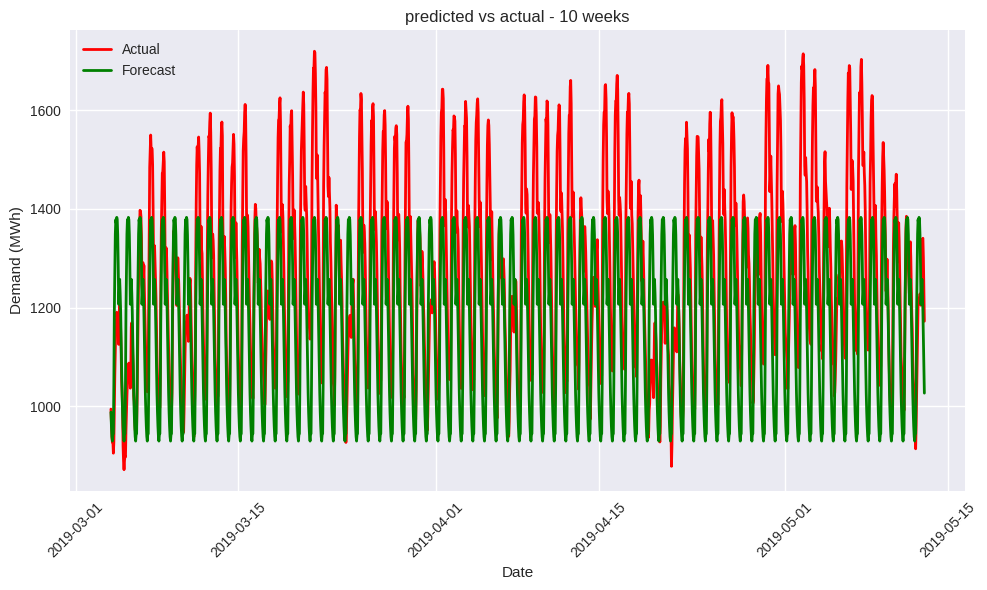
\includegraphics[width=\linewidth]{Chapters/images/results/ES_predicted_vs_actual_10weeks}
	\caption{ES model predicted vs actual load demand over 10 weeks}
	\label{fig:espredictedvsactual10weeks}
	
\end{minipage}
\end{figure}
 Figure \ref{fig:espredictedvsactual} shows the predicted and the actual values. This image shows that the model has learned the train data and does not adjust the prediction to the changing features.Figure \ref{fig:espredictedvsactual10weeks} further shows the generalization by the model. This is because ES models are not best suit for non linear problem sets.

\subsubsection{LSTM model results}
The LSTM model performed better than the ES model producing an MAPE value of 4.23\% and an MAE of 48.28 Mwh. LSTM models perform better because of their ability to learn context through the cell state mentioned in section \ref{sec:lstm_background}. Table \ref{tab:lstm_performance}of the results produced by the LSTM model.
\begin{table}[h]
	\centering
	\caption{LSTM Model Performance Metrics}
	\label{tab:lstm_performance}
	\begin{tabular}{lc}
		\hline
		\textbf{Metric} & \textbf{Value} \\
		\hline
		Mean Squared Error (MSE) & 4548.4186 \\
		Root Mean Squared Error (RMSE) & 67.4420 \\
		Mean Absolute Error (MAE) & 48.2793 \\
		Coefficient of Determination ($R^2$) & 0.8715 \\
		Mean Absolute Percentage Error (MAPE) & 4.2312\% \\
		\hline
	\end{tabular}
\end{table}
 The lower MSE and RMSE values indicate that this model has a better fit. The $R^2$ score of 0.8715 reflects a robust generalization performance and the model loss curves in figure \ref{fig:lstmmodel-loss} further show that the model is learning and generalizing properly.\begin{figure}[h]
 	\centering
 	\includegraphics[width=0.9\linewidth]{"Chapters/images/results/lstm_model loss"}
 	\caption{The LSTM model loss during training and validation}
 	\label{fig:lstmmodel-loss}
 \end{figure}
 
